% Evaluation
% Related with the requirements:
% Test 1: R1: pH Control: change constant's value and verify control work

\subsection{The Circuit Setup}

To setup the test environment,
four LED have been replacing by the water cycling and pH pumps.
It is important to pay attention at the maximum current draw from Arduino,
as well as the 20 milliamperes limit for each LED,
hence there are three $270\Omega$ resistors in serial with each LED,
as represented in the circuit diagram of figure \ref{fig:testCircuit}.

\begin{figure}[h!]
    \centering
    \includegraphics[width=.6\textwidth]{diagrams/testCircuit_bb.png}
    \caption{The circuit diagram used for testing the system. It respects the pump pins convention, where the pumps are replaced by LED for the sake of simplify the test}
    \label{fig:testCircuit}
\end{figure}

\begin{figure}[h!]
    \centering
    \includegraphics[width=.7\textwidth]{img/testCircuitPhoto3.png}
    \caption{The components used in the experiment.
    1) Male-female jumper cables to physically separate different FSM LED;
    2) Normal breadboard cables;
    3) A mobile phone to record the real-time video;
    4) A breadboard;
    5) Four $270\Omega$ resistors;
    6) An Arduino Uno Revision 3 programming platform;
    7) USB cable for serial communication and power supply;
    8) Four LED with contrasting colors: Red, Green, Blue and Yellow;
}
    \label{fig:photoCircuit}
\end{figure}

\subsection{A Graphical User Interface}

For the sake of making the unit tests to be shown in a written report,
a simple Graphical User Interface (GUI) has been implemented using Processing.
Processing is a simple programming language which is integrated with OpenGL,
Java and Serial communication.
So it is a reliable choice to display and transmit Serial data from/to Arduino within the computer screen.
But,
instead of being a monitoring-only GUI,
the Processing provides built-in functions to make mouse interactions easily,
hence the tests could be made faster.
The GUI program converses with a special Arduino program,
which is a merge of the code from \ref{lst:wcReview} and \ref{lst:ph1}.

\subsubsection{A Simple Serial Communication Protocol}

To make the Arduino and Processing exchange messages and understand those exact meaning intended,
a simple protocol has been made allowing a simple handshake and several simple commands,
which can be interpreted as text messages.

\begin{table}[h!]
\centering
\caption{Arduino--Processing Commands}
\label{tab:commands}
\begin{tabular}[h]{|l|l|l|}
    \hline
    \textbf{Command}     & \textbf{Source}    & \textbf{Meaning}
    \\\hline
    A           & Arduino    & Try to establish contact with a client
    \\\hline
    ACK         & Arduino    & Handshake is done
    \\\hline
    C           & Arduino    & The water cycling pump has been toggled
    \\\hline
    p<float>    & Processing & Send a hypothetical pH value of <float> \\ 
                &            & to simulate how the system responds to it
    \\\hline
    r           & Processing & Establish Contact or Retry Establishment
    \\\hline
\end{tabular}
\end{table}

The figure \ref{fig:sdProtocol} is a sequence diagram which describes in detail how the communication is made.
Note that the messages derived from $1$ are regarded to the connection phases,
and the messages derived from $2$ groups every command related to pH Control.

\begin{figure}[h!]
    \centering
    \includegraphics[width=.5\textwidth]{diagrams/protocolSD.png}
    \caption{A sequence diagram depicting a connection between Arduino and Processing powered GUI followed by a pH Control request}
    \label{fig:sdProtocol}
\end{figure}

A screenshot of the serial monitor has been made to show a real example of the communication,
as follows in the figure \ref{fig:serialMonitor},
one can see that the pH of 7.5 was requested and the response is composed by 14 messages updating the pH value for each second,
with an extra one to finish the response packet and let Arduino to receive new pH values.
This relative high number of updates are expected,
since there the pH variation is simulated like as described in section \ref{sec:video}.

\begin{figure}[h!]
    \centering
    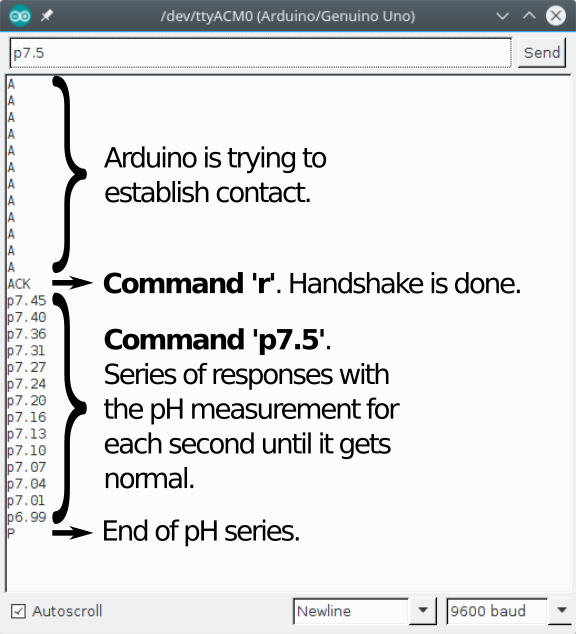
\includegraphics[width=.4\textwidth]{img/serialMon.png}
    \caption{The Arduino IDE Serial Monitor showing raw serial data}
    \label{fig:serialMonitor}
\end{figure}

\paragraph{Error Handling}

A classic retry connection option is available to make the interface more usable,
when the user has forgotten to connect the Arduino to the USB port,
for example.

\paragraph{IP Camera Support}
With the usage of the IP Capture library \cite{ipcapture_2016} and an Android App,
the author's camera turned into a IP Camera which can be displayed in real-time within the GUI.


\subsubsection{A Video Overview}
\label{sec:video}
A screencast has been uploaded at \href{https://drive.google.com/file/d/0B4QCTJgfjhCbc3FqTmVNSEE1U2c/view?usp=sharing}{Google Drive},\footnote{https://drive.google.com/file/d/0B4QCTJgfjhCbc3FqTmVNSEE1U2c/view?usp=sharing}
where the LED lights represent the FSM's states as described in table \ref{tab:leds}.
Their location is showed in figure \ref{fig:g4p}.

\begin{table}
    \centering
    \caption{Circuit LED turned on representation}
    \label{tab:leds}

    \begin{tabular}[h]{|l|l|}
        \hline
        Green   & Water is being cycled by a pump
        \\\hline
        Red     & pH is below the minimum desired value
        \\\hline
        Blue    & pH is in the normal range
        \\\hline
        Yellow  & pH is above the minimum desired value
        \\\hline

    \end{tabular}
\end{table}

\begin{figure}[h!]
    \centering
    \includegraphics[width=.7\textwidth]{img/gui4.png}
    \caption{A screenshot of the GUI with all four LED highlighted}
    \label{fig:g4p}
\end{figure}

Concerning the pH variation during time -- when two solution with different pH are blended --,
a simple and rough approximation has been made, 
based on the expectation that the pH will vary lesser and lesser during time,
as the tank solution's pH becomes closer to the pH of the controlling pH tanks.

Moreover,
to still being concise,
the water cycling parameters have been reduced:
one hour is 12 seconds and a quarter of a hour is 3 seconds.

The water cycle counter increments when the pump turns off,
in other words,
when the LED is turned off in the simulation.
The pH level terminology follows what is expected to be a desirable pH range in \ref{req2}.
